\documentclass[handout]{beamer}
% \documentclass{beamer}

%%
%%
%%
% From http://tex.stackexchange.com/questions/2072/beamer-navigation-circles-without-subsections
% Solution #2 or 3:
% \usepackage{etoolbox}
% \makeatletter
% % replace the subsection number test with a test that always returns true
% \patchcmd{\slideentry}{\ifnum#2>0}{\ifnum2>0}{}{\@error{unable to patch}}%
% \makeatother
% Solution #1:
\usepackage{remreset}% tiny package containing just the \@removefromreset command
\makeatletter
\@removefromreset{subsection}{section}
\makeatother
\setcounter{subsection}{1}


\usepackage{etex}
\usepackage{pgf}
\usepackage{tikz}
\usepackage{url}
\usepackage{amsmath}
\usepackage{color}
% \definecolor{red}{rgb}{1,0,0}
\usepackage{ulem}
% \usepackage{booktabs}
\usepackage{colortbl,booktabs}
\renewcommand*{\thefootnote}{\fnsymbol{footnote}}
\usepackage{fancybox}
\usepackage[framemethod=TikZ]{mdframed}
\mdfdefinestyle{FactStyle}{%
  outerlinewidth=0.5,
  roundcorner=1pt,
  leftmargin=1cm,
  linecolor=blue,
  outerlinecolor=blue!70!black,
  backgroundcolor=yellow!40
}
\usepackage{cancel}

  \newcommand\Warning{%
    \makebox[2.4em][c]{%
      \makebox[0pt][c]{\raisebox{.2em}{\Large!}}%
      \makebox[0pt][c]{\color{red}\Huge$\bigtriangleup$}}}%

\usepackage{stackengine}
\usepackage{scalerel}
\usepackage{xcolor}
  \newcommand\dangersign[1][2ex]{%
    \renewcommand\stacktype{L}%
    \scaleto{\stackon[1.3pt]{\color{red}$\triangle$}{\tiny !}}{#1}%
  }



\usepackage{dcolumn}
\newcolumntype{d}[1]{D{.}{.}{#1}}

% From
% http://tex.stackexchange.com/questions/109900/how-can-i-box-multiple-aligned-equations
\usepackage{empheq}
\usepackage{tcolorbox}  \newtcbox{\othermathbox}[1][]{%
  nobeforeafter, tcbox raise base, 
  colback=black!10, colframe=red!30, 
  left=1em, top=0.5em, right=1em, bottom=0.5em}

\newcommand\blue{\color{blue}}
\newcommand\red{\color{red}}
\newcommand\green{\color{green!75!black}}
\newcommand\purple{\color{purple}}
\newcommand\bluegreen{\color{blue!75!green}}
\newcommand\orange{\color{orange}}
\newcommand\redgreen{\color{red!50!green}}
\newcommand\grey{\color{black}}
\newcommand\gap{\vspace{.1in}}
\newcommand\nb{${\red\bullet}\ $}
\newcommand\halfgap{\vspace{.05in}}
\newcommand\divideline{\line(1,0){352}}
\usepackage{marvosym} % for \Smiley

\newcommand{\bluealert}[1]{{\blue\textbf{#1}}}

% \usepackage{beamerthemesplit} %Key package for beamer
\usetheme{Singapore}
% \usetheme{Szeged}
% \usetheme{Garfield}
% \usetheme{CambridgeUS}
% \usenavigationsymbolstemplate{} %Gets rid of slide navigation symbols


\setbeamercolor{separation line}{use=structure,bg=structure.fg!50!bg}
% \begin{beamercolorbox}[colsep=0.5pt]
%   {upper separation line foot}
% \end{beamercolorbox}



\makeatletter
\setbeamertemplate{footline}
{
  \leavevmode%
  \hbox{%
% \begin{beamercolorbox}[colsep=0.5pt]
%   {upper separation line foot}
% \end{beamercolorbox}


  \begin{beamercolorbox}[wd=.5\paperwidth,ht=2.25ex,dp=2ex,colsep=0.5pt]%
    {upper separation line foot}
    \usebeamerfont{author in head/foot}%
    \hspace*{2ex}\insertshortdate:\ \insertshorttitle
  \end{beamercolorbox}%
  \begin{beamercolorbox}[wd=.5\paperwidth,ht=2.25ex,dp=2ex,right]{title in head/foot}%
    \usebeamerfont{title in head/foot}
    {\insertshortauthor}\hspace*{2ex}
  \end{beamercolorbox}}%
  % \begin{beamercolorbox}[wd=.333333\paperwidth,ht=2.25ex,dp=2ex,right]{date in head/foot}%
  %   \usebeamerfont{date in head/foot}\insertshortdate{}\hspace*{2em}
  %   \insertframenumber{} / \inserttotalframenumber\hspace*{2ex} 
  % \end{beamercolorbox}%
  \vskip0pt%
}
\makeatother

\usetikzlibrary{decorations.markings}
\usetikzlibrary{arrows}


\title{Final Exam Review}
\author{Peter Garfield, UCSB Mathematics}
\date{March 15, 2017}
%\institute{}


\useinnertheme{default}

\usefonttheme{serif}
% \usecolortheme{rose}
% \usecolortheme{whale}
% \usecolortheme{orchid}
\usecolortheme{crane}
% \usecolortheme{dolphin}


%TEMPLATE
\setbeamertemplate{navigation symbols}{}

\setbeamertemplate{note page}[compress]

\setbeamertemplate{frametitle}{
  \vspace{0.5em}
  % \begin{centering}
  {\huge\blue\textbf{\textmd{\insertframetitle}}}
  \par
  % \end{centering}
}

% From http://tex.stackexchange.com/questions/7032/good-way-to-make-textcircled-numbers:
\newcommand*\circled[1]{\tikz[baseline=(char.base)]{\node[shape=circle,draw,fill=orange,inner sep=1pt] (char) {#1};}} 
% \renewcommand{\labelenumi}{\circled{\textbf{\arabic{enumi}}}}

\let\olddescription\description
\let\oldenddescription\enddescription
\usepackage{enumitem}
\let\description\olddescription
\let\enddescription\oldenddescription

% \usepackage[loadonly]{enumitem}
\setlist[enumerate,1]{label=\colorbox{orange}{\arabic*.},font=\bfseries}
%\setlist[enumerate,2]{label=\colorbox{blue!25}{(\alph*)},font=\bfseries}
% \setlist[enumerate,1]{label=\arabic*.,font=\bfseries}
\setlist[itemize,1]{label=\red$\bullet$}
\setlist[itemize,2]{label=\blue$\bullet$}

\newcommand\answer[1]{\fbox{#1}}
% \renewcommand\answer[1]{}

\newcommand{\antilog}{\operatorname{antilog}}







\title{}
\title{Ch.\ 7: Logs \& Antilogs}
\date{April 26, 2017}


\begin{document}
\small

\section*{Administration}

\frame{
  \frametitle{Office Hours!}
  % \ \vspace*{0.25in}

  {\Large{}Instructor:}\\
  \ \hspace*{0.2in} Trevor Klar, \url{trevorklar@math.ucsb.edu}\\[0.25em]

  {\Large{}Office Hours:}\\
  \ \hspace*{0.2in} Mondays 2--3\textsc{pm}\\
  \ \hspace*{0.2in} Tuesdays 10:30--11:30\textsc{am}\\
  \ \hspace*{0.2in} Thursdays 1--2\textsc{pm}\\
  \ \hspace*{0.2in} or by appointment \\[0.25em]

  {\Large{}Office:}\\
  \ \hspace*{0.2in} South Hall 6431X (Grad Tower, 6th floor, blue side, first door on the right)\\[0.5em]

  \copyright\ 2017\ Daryl Cooper, Trevor Klar

  % \vspace*{2in}
}

\if0
\frame{
  \frametitle{Exam 1 Results}

  {\Large Average: 13.60 out of 16 (85\%)}
  \bigskip
  \pause

  If you scored \alert{under 10}\ (or simply feel the need), please
  come talk to me or your TA to talk about how you can study and
  improve.
  \bigskip

}  
\fi

\section*{Logarithms}

\frame{
  \frametitle{Remember: Logarithms}
  \begin{empheq}[box=\othermathbox]{align*}
    \text{$\log(y)$ is how may tens you multiply together to get $y$}
  \end{empheq}
  \pause 

  \begin{empheq}[box=\othermathbox]{align*}
    10^{\log(y)} & = y
  \end{empheq}

  \uncover<2->{%
    \begin{align*}
      \log({\blue 100}) 
      & \only<2>{ = ?}%
      \uncover<3->{%
      = {\red 2}
        \qquad\text{because}\quad 
       10^{\red 2} ={\blue 100}
        }
    \end{align*}
  }

  \uncover<4->{%
    {\large\alert{You Try It:}}
    $\log({\blue 100,000}) = ?$
    \begin{center}
      A$= 2$
      \quad 
      B$= 3$
      \quad 
      C$= 4$
      \quad 
      D$= 5$
      \quad 
      E$ = 6$
      \quad
      \uncover<5>{\fbox{D}}
    \end{center}
  }
}




\frame{
  \frametitle{A Few More:}

$\log({0.001}) = ?$
\begin{center}
  A$=3$
  \quad 
  B$ = 0$
  \quad 
  C$ =0.001$
  \quad 
  D$ = -2$
  \quad 
  E$ = -3$ 
  \quad
  \pause
  \fbox{E}
\end{center}
\gap

$\log(100\times1000)=?$
\begin{center}
  A$ = 6$
  \quad 
  B$ = 5$
  \quad 
  C$ = 3$
  \quad 
  D$ = 9$
  \quad 
  E$ = -5$
  \pause
  \quad
  \fbox{B}
\end{center}
\gap

$\log(100/1000)=?$
\begin{center}
  A$ =-1$
  \quad 
  B$ = 0$
  \quad 
  C$ = 1$
  \quad 
  D$ = -3$
  \quad 
  E$ = -5$
  \pause
  \quad
  \fbox{A}
\end{center}
\gap

\gap How confused are you ?
\begin{center}
  A = not at all\quad B = a bit\quad C = a lot\quad D = completely
\end{center}





}

\frame{
  \frametitle{How To Find Logarithms} 

  \begin{itemize}
  \item[\red(1)] Use a calculator: efficient but not good for {\blue
      learning} 

  \item[\red(2)] Use the graph on page 290 of textbook

  \item[\red(3)] Use table of logarithms on page 289 of textbook

  \end{itemize}
  \pause

  \gap

  Our goal: use {\red(2)}\ and {\red(3)}\ to understand: 
  \begin{center}
    {\blue logs}, {\red functions} and {\purple inverse functions}.
  \end{center}
  Our main use of logs: solving certain kinds of equation.

  Mistakes will follow unless you \alert{\emph{practice}}\ finding
  logs the old fashioned way.
  \pause
  % \vspace*{-2mm}

  \begin{minipage}{0.4\linewidth}
    \large
    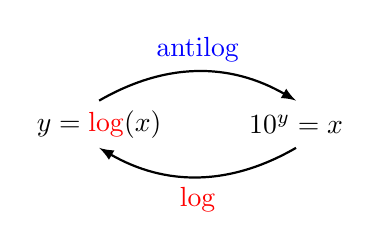
\begin{tikzpicture}[x=12.5mm,y=10mm,>=latex]
      \node at (-1,0) {$y={\red\log}(x)$};
      \node at (1,0) {$10^y=x$};
      % Connect 'em:
      \draw[thick,bend left,->,>=latex] (-1,0.3) to node [auto,midway,blue] {antilog} (1,0.3) ;
      \draw[thick,bend left,->,>=latex] (1,-0.3) to node [auto,midway,red] {log} (-1,-0.3) ;
    \end{tikzpicture}
  \end{minipage}
  \begin{minipage}{0.55\linewidth}
    \large
    {\red$\log$}\ is the inverse function of {\blue{}antilog} \\[0.2em]
    %
    {\blue{}antilog}\ is another name for\\ the {\blue$10$-to-the-power function:}\\[-1em]
    \begin{equation*}
      \text{\blue{}antilog}(y) = 10^y.
    \end{equation*}

  \end{minipage}

}

\frame{

{\tiny
\begin{equation*}
\begin{tabular}{*{11}{c}}
$x$ & 0.00 & 0.01 & 0.02 & \only<2>{\cellcolor{blue!75}}0.03 & 0.04 & 0.05 & 0.06\only<3>{\cellcolor{red!75}} & 0.07 & 0.08 & 0.09 \\ \toprule
1.0 & 0.0000 & 0.0043 & 0.0086 & 0.0128 & 0.0170 & 0.0212 & 0.0253 & 0.0294 & 0.0334 & 0.0374 \\
\rowcolor[gray]{0.75}
1.1 & 0.0414 & 0.0453 & 0.0492 & 0.0531 & 0.0569 & 0.0607 & 0.0645 & 0.0682 & 0.0719 & 0.0755 \\
1.2 & 0.0792 & 0.0828 & 0.0864 & 0.0899 & 0.0934 & 0.0969 & 0.1004 & 0.1038 & 0.1072 & 0.1106 \\
\rowcolor[gray]{0.75}
1.3 & 0.1139 & 0.1173 & 0.1206 & 0.1239 & 0.1271 & 0.1303 & 0.1335 & 0.1367 & 0.1399 & 0.1430 \\
1.4 & 0.1461 & 0.1492 & 0.1523 & 0.1553 & 0.1584 & 0.1614 & 0.1644 & 0.1673 & 0.1703 & 0.1732 \\
\rowcolor[gray]{0.75}
1.5 & 0.1761 & 0.1790 & 0.1818 & 0.1847 & 0.1875 & 0.1903 & 0.1931 & 0.1959 & 0.1987 & 0.2014 \\
1.6 & 0.2041 & 0.2068 & 0.2095 & 0.2122 & 0.2148 & 0.2175 & 0.2201 & 0.2227 & 0.2253 & 0.2279 \\
\rowcolor[gray]{0.75}
1.7 & 0.2304 & 0.2330 & 0.2355 & 0.2380 & 0.2405 & 0.2430 & 0.2455 & 0.2480 & 0.2504 & 0.2529 \\
1.8 & 0.2553 & 0.2577 & 0.2601 & 0.2625 & 0.2648 & 0.2672 & 0.2695 & 0.2718 & 0.2742 & 0.2765 \\
\rowcolor[gray]{0.75}\only<3>{\cellcolor{red!75}}%
1.9 & 0.2788 & 0.2810 & 0.2833 & 0.2856 & 0.2878 & 0.2900 & \only<3>{\cellcolor{red!90}}0.2923 & 0.2945 & 0.2967 & 0.2989 \\
2.0 & 0.3010 & 0.3032 & 0.3054 & 0.3075 & 0.3096 & 0.3118 & 0.3139 & 0.3160 & 0.3181 & 0.3201 \\
\rowcolor[gray]{0.75}
2.1 & 0.3222 & 0.3243 & 0.3263 & 0.3284 & 0.3304 & 0.3324 & 0.3345 & 0.3365 & 0.3385 & 0.3404 \\
2.2 & 0.3424 & 0.3444 & 0.3464 & 0.3483 & 0.3502 & 0.3522 & 0.3541 & 0.3560 & 0.3579 & 0.3598 \\
\rowcolor[gray]{0.75}
2.3 & 0.3617 & 0.3636 & 0.3655 & 0.3674 & 0.3692 & 0.3711 & 0.3729 & 0.3747 & 0.3766 & 0.3784 \\
2.4 & 0.3802 & 0.3820 & 0.3838 & 0.3856 & 0.3874 & 0.3892 & 0.3909 & 0.3927 & 0.3945 & 0.3962 \\
\rowcolor[gray]{0.75}
2.5 & 0.3979 & 0.3997 & 0.4014 & 0.4031 & 0.4048 & 0.4065 & 0.4082 & 0.4099 & 0.4116 & 0.4133 \\
2.6 & 0.4150 & 0.4166 & 0.4183 & 0.4200 & 0.4216 & 0.4232 & 0.4249 & 0.4265 & 0.4281 & 0.4298 \\
\rowcolor[gray]{0.75}\only<2>{\cellcolor{blue!75}}%
2.7 & 0.4314 & 0.4330 & 0.4346 & \only<2>{\cellcolor{blue!90}}0.4362 & 0.4378 & 0.4393 & 0.4409 & 0.4425 & 0.4440 & 0.4456 \\
2.8 & 0.4472 & 0.4487 & 0.4502 & 0.4518 & 0.4533 & 0.4548 & 0.4564 & 0.4579 & 0.4594 & 0.4609 \\
\rowcolor[gray]{0.75}
2.9 & 0.4624 & 0.4639 & 0.4654 & 0.4669 & 0.4683 & 0.4698 & 0.4713 & 0.4728 & 0.4742 & 0.4757 \\
3.0 & 0.4771 & 0.4786 & 0.4800 & 0.4814 & 0.4829 & 0.4843 & 0.4857 & 0.4871 & 0.4886 & 0.4900 \\
\rowcolor[gray]{0.75}
3.1 & 0.4914 & 0.4928 & 0.4942 & 0.4955 & 0.4969 & 0.4983 & 0.4997 & 0.5011 & 0.5024 & 0.5038 \\
3.2 & 0.5051 & 0.5065 & 0.5079 & 0.5092 & 0.5105 & 0.5119 & 0.5132 & 0.5145 & 0.5159 & 0.5172 \\
\rowcolor[gray]{0.75}
3.3 & 0.5185 & 0.5198 & 0.5211 & 0.5224 & 0.5237 & 0.5250 & 0.5263 & 0.5276 & 0.5289 & 0.5302 \\
3.4 & 0.5315 & 0.5328 & 0.5340 & 0.5353 & 0.5366 & 0.5378 & 0.5391 & 0.5403 & 0.5416 & 0.5428 \\
\end{tabular}
\end{equation*}
}

\uncover<2->{%
  Use table \alert{\emph{forwards}}\ to find logs: {\blue$\log(2.73) \approx 0.4362$}
}
\smallskip

\uncover<3->{%
  Use table \alert{\emph{backwards}}\ to find powers of $10$: {\red$10^{0.2923} \approx 1.96$}
}
\bigskip
\bigskip

}


\frame{

{\tiny
\begin{equation*}
\begin{tabular}{*{11}{c}}
$x$ & 0.00 & 0.01 & 0.02 & 0.03 & 0.04 & 0.05 & 0.06 & 0.07 & 0.08 & 0.09 \\ \toprule
1.0 & 0.0000 & 0.0043 & 0.0086 & 0.0128 & 0.0170 & 0.0212 & 0.0253 & 0.0294 & 0.0334 & 0.0374 \\
\rowcolor[gray]{0.75}
1.1 & 0.0414 & 0.0453 & 0.0492 & 0.0531 & 0.0569 & 0.0607 & 0.0645 & 0.0682 & 0.0719 & 0.0755 \\
1.2 & 0.0792 & 0.0828 & 0.0864 & 0.0899 & 0.0934 & 0.0969 & 0.1004 & 0.1038 & 0.1072 & 0.1106 \\
\rowcolor[gray]{0.75}
1.3 & 0.1139 & 0.1173 & 0.1206 & 0.1239 & 0.1271 & 0.1303 & 0.1335 & 0.1367 & 0.1399 & 0.1430 \\
1.4 & 0.1461 & 0.1492 & 0.1523 & 0.1553 & 0.1584 & 0.1614 & 0.1644 & 0.1673 & 0.1703 & 0.1732 \\
\rowcolor[gray]{0.75}
1.5 & 0.1761 & 0.1790 & 0.1818 & 0.1847 & 0.1875 & 0.1903 & 0.1931 & 0.1959 & 0.1987 & 0.2014 \\
1.6 & 0.2041 & 0.2068 & 0.2095 & 0.2122 & 0.2148 & 0.2175 & 0.2201 & 0.2227 & 0.2253 & 0.2279 \\
\rowcolor[gray]{0.75}
1.7 & 0.2304 & 0.2330 & 0.2355 & 0.2380 & 0.2405 & 0.2430 & 0.2455 & 0.2480 & 0.2504 & 0.2529 \\
1.8 & 0.2553 & 0.2577 & 0.2601 & 0.2625 & 0.2648 & 0.2672 & 0.2695 & 0.2718 & 0.2742 & 0.2765 \\
\rowcolor[gray]{0.75}
1.9 & 0.2788 & 0.2810 & 0.2833 & 0.2856 & 0.2878 & 0.2900 & 0.2923 & 0.2945 & 0.2967 & 0.2989 \\
2.0 & 0.3010 & 0.3032 & 0.3054 & 0.3075 & 0.3096 & 0.3118 & 0.3139 & 0.3160 & 0.3181 & 0.3201 \\
\rowcolor[gray]{0.75}
2.1 & 0.3222 & 0.3243 & 0.3263 & 0.3284 & 0.3304 & 0.3324 & 0.3345 & 0.3365 & 0.3385 & 0.3404 \\
2.2 & 0.3424 & 0.3444 & 0.3464 & 0.3483 & 0.3502 & 0.3522 & 0.3541 & 0.3560 & 0.3579 & 0.3598 \\
\rowcolor[gray]{0.75}
2.3 & 0.3617 & 0.3636 & 0.3655 & 0.3674 & 0.3692 & 0.3711 & 0.3729 & 0.3747 & 0.3766 & 0.3784 \\
2.4 & 0.3802 & 0.3820 & 0.3838 & 0.3856 & 0.3874 & 0.3892 & 0.3909 & 0.3927 & 0.3945 & 0.3962 \\
\rowcolor[gray]{0.75}
2.5 & 0.3979 & 0.3997 & 0.4014 & 0.4031 & 0.4048 & 0.4065 & 0.4082 & 0.4099 & 0.4116 & 0.4133 \\
2.6 & 0.4150 & 0.4166 & 0.4183 & 0.4200 & 0.4216 & 0.4232 & 0.4249 & 0.4265 & 0.4281 & 0.4298 \\
\rowcolor[gray]{0.75}
2.7 & 0.4314 & 0.4330 & 0.4346 & 0.4362 & 0.4378 & 0.4393 & 0.4409 & 0.4425 & 0.4440 & 0.4456 \\
2.8 & 0.4472 & 0.4487 & 0.4502 & 0.4518 & 0.4533 & 0.4548 & 0.4564 & 0.4579 & 0.4594 & 0.4609 \\
\rowcolor[gray]{0.75}
2.9 & 0.4624 & 0.4639 & 0.4654 & 0.4669 & 0.4683 & 0.4698 & 0.4713 & 0.4728 & 0.4742 & 0.4757 \\
3.0 & 0.4771 & 0.4786 & 0.4800 & 0.4814 & 0.4829 & 0.4843 & 0.4857 & 0.4871 & 0.4886 & 0.4900 \\
\rowcolor[gray]{0.75}
3.1 & 0.4914 & 0.4928 & 0.4942 & 0.4955 & 0.4969 & 0.4983 & 0.4997 & 0.5011 & 0.5024 & 0.5038 \\
3.2 & 0.5051 & 0.5065 & 0.5079 & 0.5092 & 0.5105 & 0.5119 & 0.5132 & 0.5145 & 0.5159 & 0.5172 \\
\rowcolor[gray]{0.75}
3.3 & 0.5185 & 0.5198 & 0.5211 & 0.5224 & 0.5237 & 0.5250 & 0.5263 & 0.5276 & 0.5289 & 0.5302 \\
3.4 & 0.5315 & 0.5328 & 0.5340 & 0.5353 & 0.5366 & 0.5378 & 0.5391 & 0.5403 & 0.5416 & 0.5428 \\
\end{tabular}
\end{equation*}
}
  

$\log(2.372)$\ is\
\begin{center}
  A$\approx 0.3729$
  \quad 
  B$\approx 0.3747$
  \quad 
  C$\approx 0.3766$
  \pause
  \quad\fbox{B} 
\end{center}
\bigskip


}

\frame{

  \begin{center}
    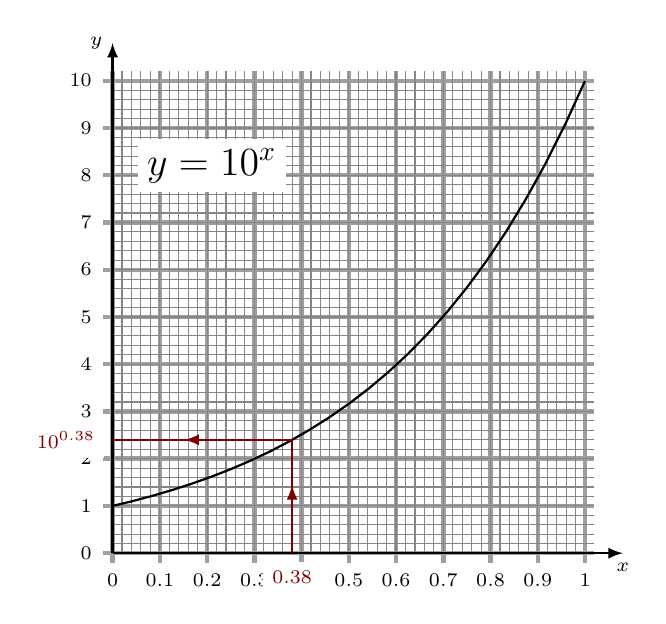
\begin{tikzpicture}[x=60mm,y=6mm,>=latex]
      \foreach \x in {0,0.1,0.2,0.3,0.4,0.5,0.6,0.7,0.8,0.9,1}
      {
        \draw[ultra thick,gray!75] (\x,10.2) -- (\x,-0.2) node[black,below] {$\scriptstyle\x$};
      }
      \foreach \y in {0,1,...,10} 
      {
        \draw[ultra thick,gray!75] (1.02,\y) -- (-0.02,\y) node[black,left] {$\scriptstyle\y$};
      }
      \foreach \k in {2,4,...,98}
      {
        \draw[thin,gray!95] ({\k/100},10.2) -- ({\k/100},0);
        \draw[thin,gray!95] (1.02,{\k/10}) -- (0,{\k/10});
      }
      % 
      \draw[thick,black,->] (0,0) -- (1.08,0) node[below] {$\scriptstyle{}x$};
      \draw[thick,black,->] (0,0) -- (0,10.8) node[left] {$\scriptstyle{}y$};
      \draw[thick,black] plot[domain=0:1] (\x,{10^(\x)});
      \node[black,fill=white] at (0.21,8.2) {\Large$y=10^x$};
      \uncover<2->{%
        \draw[thick,red!50!black] (0.38,0) -- (0.38,{10^(0.38)}) -- (0,{10^(0.38)});
        \draw[thick,red!50!black,->] (0.38,0) -- (0.38,{10^(0.38)*0.6});
        \draw[thick,red!50!black,->] (0.38,{10^(0.38)}) -- ({0.38*0.4},{10^(0.38)});
        \node[red!50!black,fill=white,below,yshift=-1mm] at (0.38,0) {$\scriptstyle0.38$};
        \node[red!50!black,fill=white,left,xshift=-1mm] at (0,{10^(0.38)}) {$\scriptstyle10^{0.38}$};
      }
    \end{tikzpicture}
  \end{center}

  Use the graph % on page 290 of your textbook 
  and a ruler to find
  $10^{0.38}$:
  \begin{center}
    A$\approx 2.1$
    \quad 
    B$\approx 2.2$
    \quad 
    C$\approx 2.3$
    \quad 
    D$\approx 2.4$
    \quad 
    E$ \approx 2.6$    
    \quad
    \uncover<2->{\fbox{D}}
  \end{center}




}


\frame{

  \begin{center}
    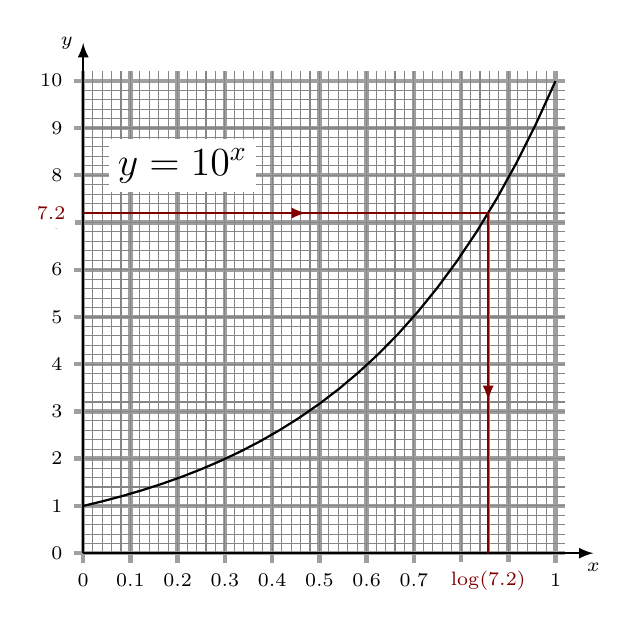
\begin{tikzpicture}[x=60mm,y=6mm,>=latex]
      \foreach \x in {0,0.1,0.2,0.3,0.4,0.5,0.6,0.7,0.8,0.9,1}
      {
        \draw[ultra thick,gray!75] (\x,10.2) -- (\x,-0.2) node[black,below] {$\scriptstyle\x$};
      }
      \foreach \y in {0,1,...,10} 
      {
        \draw[ultra thick,gray!75] (1.02,\y) -- (-0.02,\y) node[black,left] {$\scriptstyle\y$};
      }
      \foreach \k in {2,4,...,98}
      {
        \draw[thin,gray!95] ({\k/100},10.2) -- ({\k/100},0);
        \draw[thin,gray!95] (1.02,{\k/10}) -- (0,{\k/10});
      }
      % 
      \draw[thick,black,->] (0,0) -- (1.08,0) node[below] {$\scriptstyle{}x$};
      \draw[thick,black,->] (0,0) -- (0,10.8) node[left] {$\scriptstyle{}y$};
      \draw[thick,black] plot[domain=0:1] (\x,{10^(\x)});
      \node[black,fill=white] at (0.21,8.2) {\Large$y=10^x$};
      \uncover<2->{%
        \draw[thick,red!50!black] (0,7.2) -- ({ln(7.2)/ln(10)},7.2) -- ({ln(7.2)/ln(10)},0);
        \draw[thick,red!50!black,->] (0,7.2) -- ({0.55*ln(7.2)/ln(10)},7.2);
        \draw[thick,red!50!black,->] ({ln(7.2)/ln(10)},7.2) -- ({ln(7.2)/ln(10)},{0.45*7.2});
        \node[red!50!black,fill=white,below,yshift=-1mm] at ({ln(7.2)/ln(10)},0) {$\scriptstyle\log(7.2)$};
        \node[red!50!black,fill=white,left,xshift=-1mm] at (0,7.2) {$\scriptstyle7.2$};
      }
    \end{tikzpicture}
  \end{center}

  Use the graph \alert{\emph{backwards}}\ % on page 290 of your textbook 
  and a ruler to find $\log(7.2)$:
  \begin{center}
    A$\approx 0.81$
    \quad 
    B$\approx 0.82$
    \quad 
    C$\approx 0.83$
    \quad 
    D$\approx 0.84$
    \quad 
    E$=0.86$
    \quad 
    \uncover<2->{\fbox{E}}
  \end{center}
}

\frame{

\gap Do you have questions about using the graph of $y=10^x$ ?\\
A = lots\quad B = a few\quad C = one\quad D = none\quad E = move on already!

\gap
\pause
Do you have questions about using the table of logs on page 289 ?\\
A = lots\quad B = a few\quad C = one\quad D = none\quad E = move on already!

\gap
\pause

\begin{center}
  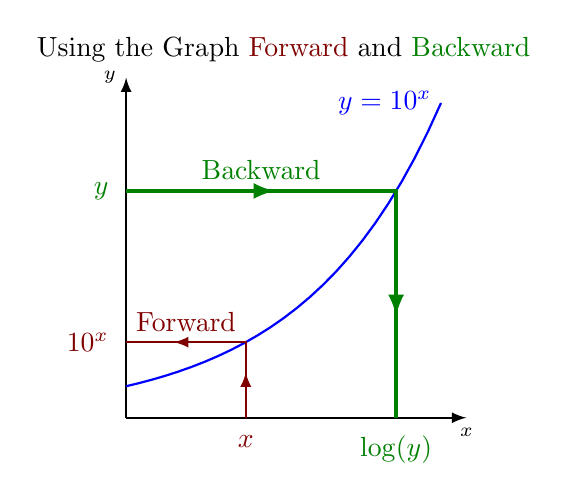
\begin{tikzpicture}[x=40mm,y=4mm,>=latex,baseline=15]
    % \foreach \x in {0,0.1,0.2,0.3,0.4,0.5,0.6,0.7,0.8,0.9,1}
    % {
    % \draw[ultra thick,gray!75] (\x,10.2) -- (\x,-0.2) node[black,below] {$\scriptstyle\x$};
    % }
    %   \foreach \y in {0,1,...,10} 
    %   {
    %   \draw[ultra thick,gray!75] (1.02,\y) -- (-0.02,\y) node[black,left] {$\scriptstyle\y$};
    % }
    %   \foreach \k in {2,4,...,98}
    %   {
    %   \draw[thin,gray!95] ({\k/100},10.2) -- ({\k/100},0);
    %   \draw[thin,gray!95] (1.02,{\k/10}) -- (0,{\k/10});
    % }
    %   
    \draw[thick,black,->] (0,0) -- (1.08,0) node[below] {$\scriptstyle{}x$};
    \draw[thick,black,->] (0,0) -- (0,10.8) node[left] {$\scriptstyle{}y$};
    \draw[thick,blue] plot[domain=0:1] (\x,{10^(\x)});
    % \node[black,fill=white] at (0.21,8.2) {\Large$y=10^x$};
    \node[left,blue] at (1,10) {$y=10^x$};
    \draw[ultra thick,green!50!black] (0,7.2) -- ({ln(7.2)/ln(10)},7.2) node[midway,above] {Backward} -- ({ln(7.2)/ln(10)},0);
    \draw[ultra thick,green!50!black,->] (0,7.2) -- ({0.55*ln(7.2)/ln(10)},7.2);
    \draw[ultra thick,green!50!black,->] ({ln(7.2)/ln(10)},7.2) -- ({ln(7.2)/ln(10)},{0.45*7.2});
    \node[green!50!black,fill=white,below,yshift=-1mm] at ({ln(7.2)/ln(10)},0) {$\log(y)$};
    \node[green!50!black,fill=white,left,xshift=-1mm] at (0,7.2) {$y$};
    \draw[thick,red!50!black] (0.38,0) -- (0.38,{10^(0.38)}) -- (0,{10^(0.38)}) node[midway,above] {Forward};
    \draw[thick,red!50!black,->] (0.38,0) -- (0.38,{10^(0.38)*0.6});
    \draw[thick,red!50!black,->] (0.38,{10^(0.38)}) -- ({0.38*0.4},{10^(0.38)});
    \node[red!50!black,fill=white,below,yshift=-1mm] at (0.38,0) {$x$};
    \node[red!50!black,fill=white,left,xshift=-1mm] at (0,{10^(0.38)}) {$10^{x}$};
    \node[above] at (0.5,11) {Using the Graph {\color{red!50!black}{}Forward}\ and {\color{green!50!black}{}Backward}};
  \end{tikzpicture}
  \hspace*{0.25in}
  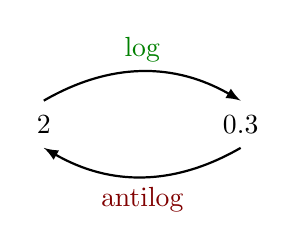
\begin{tikzpicture}[x=12.5mm,y=10mm,>=latex]
    \node at (-1,0) {$2$};
    \node at (1,0) {$0.3$};
    % Connect 'em:
    \draw[thick,bend left,->,>=latex] (-1,0.3) to node [auto,midway,green!50!black] {log} (1,0.3) ;
    \draw[thick,bend left,->,>=latex] (1,-0.3) to node [auto,midway,red!50!black] {antilog} (-1,-0.3) ;
  \end{tikzpicture}


\end{center}



}


\frame{
  \frametitle{Summary}
  \begin{itemize}
  \item ${\blue \log}(y)$ is how many tens you multiply to get y

  \item {\blue log} is the {\purple inverse function} to {\red antilog}.\\
    
  \item So: method to find $x={\blue \log}(y)$ is the {\purple opposite} of  method to find $y=10^x$ 

  \end{itemize}
  \vspace*{-1em}
  \pause

  \divideline 

  Use the graph $y=10^x$  {\blue forwards} to find $10^x.$ This means
  to find $10^{0.38}$ {\red start at $x=0.38$ on $x$-axis}. Using
  graph as intended. 
  \halfgap

  Use graph {\blue backwards} to find $\log(y).$ This means to find
  $\log(7.2)$ {\red start at $y=7.2$ on the $y$-axis}. 
  \pause 

  \divideline

  Same deal with log tables. Use the tables {\red forwards} to find
  $log(2.73).$ This means {\red find $2.73$ in the left column/top
    row} and the answer $log(2.73)=0.4362$ is in the middle of the
  table.
  \gap
  
  Use the table {\red backwards} to find $10^{0.2923}.$ This means
  {\red hunt through the middle of the table} until you find $0.2932$
  then $10^{0.2932}=1.96$ is in the left column/top row.

}

\section*{Properties of Logs}

\frame{
  \frametitle{Key Fact Of Logs}

  \begin{empheq}[box=\othermathbox]{align*}
    \text{First Law of Logs\qquad $\log(a{\blue\times} b) = \log(a) {\blue +}\log(b)$}
  \end{empheq}
  \gap

  This means logs convert {\blue multiplication} into {\blue addition}.\\
  \pause
  \halfgap

  Example: \qquad $\log(100{\blue\times}1000) = \log(100){\blue +}\log(1000) = 2 + 3 = 5$\\ \pause
  \gap 
  
  It is easy to \emph{understand} why the first law works:
  \gap

  log({\red a}) = (how many 10's you multiply to get {\red a})\\
  log({\red b}) = (how many 10's you multiply to get {\red b})\\ \pause
  \gap

  {\blue THEREFORE} multiplying ALL these 10s gives ${\red
    a}{\blue\times} {\red b}$ 
  \pause
  \gap 
  
  {\blue CONCLUDE} $\log({\red a}{\blue \times} {\red b})$ is this
  number of 10s: that is, $\log({\red a}){\blue +}\log({\red b})$.
  \gap 
  \pause

  \alert{Does this make sense to you?} \\ %This may change as I speak}\\
  \begin{center}
      A = Completely\quad B = mostly\quad C = a glimmer\quad D = no!
  \end{center}

}

\frame{
  \frametitle{Consquences of the Key Fact}

  We are told: $\log(2) \approx {\blue 0.3}$ (from table page 289)
  \gap

  \begin{align*}
    \log(20) 
    & = \log(10{\red \times}2)\\
    & = \log(10){\red +}\log(2)\qquad\qquad {\blue \text{we know }\log(10)=1}\\
    & \approx {\red 1} + {\blue 0.3}\\
    & \approx 1.3
  \end{align*}
  \pause

  Use this method to find $\log(200)$
  \begin{center}
    A$ = 30$
    \quad 
    B$=3$
    \quad 
    C$ = 2.3$
    \quad 
    D$=30$
    \pause
    \quad
    \fbox{\blue C}
  \end{center}

}

\frame{
  \frametitle{A few more}
  We are still told $\log(2) \approx {\blue 0.3}$ 
  \gap\ \gap

  Find $\log(0.002)$
  \begin{center}
    A$ = -3.3$
    \quad 
    B$=-2.3$
    \quad 
    C$ = -2.7$
    \quad 
    D$=-3.7$
    \pause
    \quad
    \fbox{C}
  \end{center}
  \gap

  Find $\log(2\times 10^x)$
  \begin{center}
    A$ = 2x$
    \quad 
    B$=2+x$
    \quad 
    C$ = x\log(2)$
    \quad 
    D$=10x+\log(2)$
    \quad 
    E$= x+\log(2)$
    \pause
    \fbox{E}
  \end{center}

}

\frame{
  \frametitle{A Trick!}

  The graph and the table can both be used\\  to find logs of numbers between {\blue 1} and {\blue 10}.
  \gap

  To find the log of ANY number, we move the decimal point:
  \begin{empheq}[box=\othermathbox]{equation*}
    \log(10^{\blue n}{\red\times} x) 
    = {\blue n}\,{\red+}\,\log(x)
  \end{empheq}
  \pause

  Example:
  \begin{equation*}
    \log(275.67)
    = \log(10^{\blue 2}{\red\times}2.7567) 
    =  {\blue 2}{\red+} \underbrace{ \log(2.7567)}_{\text{look this
        up!}}
  \end{equation*}
   \gap 

   Its called the {\blue MOVING DECIMAL POINT TRICK} because ${\blue
     2}$ is how many places you need to move the decimal point of
   $275.67$ to obtain a number between $1$ and $10.$  
   \gap
   
}

\frame{
  \frametitle{You Try It!}

  Use the log tables on page 289 to find $\log(5.73)$
  \begin{center}
    A = I have done it\quad B = I am confused\quad C = I don't have
    the texthere
  \end{center}
  \pause

  \fbox{\blue $\log(5.73)\approx 0.7582$} Did you get this?\\
  \begin{center}
    A = YES\quad B = No
  \end{center}
  \pause
  \gap

  What is $\log(57.3)\approx$?
  \begin{center}
    A$ = 7.582$
    \quad 
    B$ = 10+0.7582$
    \quad 
    C$ = 1+0.7582$
    \quad 
    D$ =$ OTHER
    \quad
    \pause
    \fbox{C}
  \end{center}


}
\frame{
  \frametitle{Inverses!}

logs are ``{\blue opposite} '' of exponents (inverse function of antilog)\\
So every fact about exponents corresponds to a fact about logs:

\gap

\begin{table}
\begin{tabular}{lll}
 & {\blue laws of exponents} & {\blue corresponding law of logs} \\\toprule
{\red(1)}  & $10^{\red a}\times10^{\red b} = 10^{{\red a}+{\red b}} $ & 
$\log({\blue x y})= \log({\blue x})+\log({\blue y})$ \\
{\red(2)} & $10^{\red 0} = {\blue 1}$ & $\log({\blue 1}) ={\red 0}$\\
{\red(3)} & $10^{\red -a} = 1/10^{\red a}$ & $\log({\blue 1/x}) =-\log({\blue x})$\\
{\red(4)} & $\left(10^{\red a}\right)^{\red p} = 10^{\red ap}$ & $\log({\blue x}^{\red p}) ={\red p}\log({\blue x})$\\
{\red(5)}  & $10^{\red a}/10^{\red b} = 10^{{\red a}-{\red b}} $ & $\log({\blue x/y})= \log({\blue x})-\log({\blue y})$ 
\end{tabular}
\end{table}

Example: $\log(x^a/y^b)=$?
\begin{center}
  $A = a\log(x)/(b\log(y))\qquad B = a\log(x) + b\log(y)$\\
  $C = a\log(x)-b\log(y)\quad D =(a+\log(x))-(b+\log(y))$
  \pause
  \fbox{C}   
\end{center}

}

\frame{
  \frametitle{Rule (4): $\log(x^p) = p \log(x)$}

  Explanation of {\purple (4)}
  \gap

  $\log(a\times a)=\log(a)+\log(a) = {\red 2}\log(a)$\\ \pause
  $\log(a\times a\times a)=\log(a)+\log(a) + \log(a)={\red 3}\log(a)$ \\ \pause
  \gap
  
  In general:  the number of tens you multiply to get $x^{\red p}$ is ${\red p}$ times as many tens as you multiply to get $x.$
  \gap

  What is $\log(\sqrt{x^7})$?
  \begin{center}
    $A = 7+\log(x)\quad B = (7/2)+\log(x)\quad C = 7/2\quad D = 7/2\log(x)$\quad\pause\fbox{D}
  \end{center}


}

\end{document}

\section*{Summary}

\frame{
  \frametitle{Finding the log of any number}

  {\red(1)}\ Write the number as ${\redgreen 10^n}\times$({\red number between 1 and 10})\\[0.5em]

  {\red(2)}\ Find the log of the {\red number between 1 and 10}\ using
  table or graph\\[0.5em]

  {\red(3)}\ Log is ${\redgreen{}n} + \log(\text{\red number between 1
    and 10})$
  \gap\ 
  \gap\ 
  \pause

  \alert{\large{}Example:}\ Find $\log(573)$
  \gap

  {\red(1)}\ $\log({\blue 573}) = \log({\redgreen 100}\times{\red 5.73})
  = \log({\redgreen 100}) + \log({\red 5.73}) = {\redgreen 2}+\log({\red 5.73})$
  \smallskip

  {\red(2)}\ \fbox{$\log({\red 5.73}) \approx 0.7582$}
  \smallskip

  {\red(3)}\ $\log({\blue573}) \approx 2 + 0.7582 = 2.7582$
  \gap

  Find $\log({\blue 57.3})$
  \begin{center}
    A$\approx7.582$
    \quad 
    B$\approx10+0.7582$
    \quad 
    C$\approx 1+0.7582$
    \quad 
    D\ Other
    \quad
    \pause
    \fbox{C}
  \end{center}
  \gap

  Find $\log(0.573)$
  \begin{center}
    A$\approx-1.7582$
    \quad 
    B$\approx-1+0.7582$
    \quad 
    C$\approx-0.7582$
    \quad 
    D\ Other
    \quad
    \pause
    \fbox{B}
  \end{center}

}


\frame{
  \frametitle{Finding the antilog of any number}

  \alert{Example:} ${\blue2}.306$ is not on $x$-axis of graph $y=10^x$
  or in middle of log table.  So how do you use table or graph to find
  {${\red\mbox{antilog}}({\blue 2}.306)$}?
  \gap 
  
  {\redgreen\large{}Think about it:}
  \vspace*{-2em}
  \begin{align*}
    {\red\mbox{antilog}}({\blue 2}.306)  
    & =  10^{{\blue2}.306}  \\
    \uncover<2->{%
    & = \underbrace{10^{\blue 2}}_{\text{\red{}duh!}} \times
      \underbrace{ 10^{0.306}}_{\text{\blue{}look it up!}} 
      \\ 
    }
    \uncover<3->{%
    & \approx {\blue100} \times 2.02 \\
    & = 202 
      }
  \end{align*}

  \uncover<3->{This is like the {\blue moving decimal point trick}\ for logs.}

  \uncover<4->{%
    \divideline

    From log table: $10^{0.{\green 86}}\approx7.25$. \qquad
    Use this to find ${\red\mbox{antilog}}(3.{\green 86})$ 
  }
  \uncover<5->{%
    \fbox{\blue$\approx 7250$}\\
    \begin{center}
      A$=\text{I got it right}$
      \qquad 
      B$=\text{I was close}$
      \qquad
      C$=\text{I was wrong}$
    \end{center}
  }
}


              
\end{document}

